\chapter{Strukturierte Datentypen}
\label{p:5}
%
%
Wir werden in diesem Kapitel neue M"oglichkeiten der Datenspeicherung
einf"uhren.
\begin{itemize}
  \item \textbf{Feld (array)}, \textbf{Liste}: \\
  	Zusammenfassung von  Elementen gleichen Typs.
	\index{Feld}\index{array|see{Feld}}
  \item \textbf{Struktur (struct)}: \\
  	Zusammenfassung von Komponenten verschiedenen Typs.
	\index{Struktur}\index{struct|see{Struktur}}
  \item \textbf{Union (union)}: \\
  	"Uberlagerung mehrerer Komponenten verschiedenen Typs auf
	dem gleichen Speicherplatz.
	\index{union}
  \item \textbf{Aufz"ahlungstyp (enum)} \\
  	Grunddatentyp mit frei w"ahlbarem Wertebereich.
	\index{Aufz\"ahlungstyp}\index{enum|see{Aufz\"ahlungstyp}}
\end{itemize}
%
Eine dar"uber hinausgehende, sehr gute Einf"uhrung in Algorithmen und Datenstrukturen
ist in~\cite{PombergerDobler:2008:AUD} zu finden.
%
\section{Felder}
\label{p:5.1}
%
In einem Feld/Array werden Daten (Elemente) gleichen Typs zusammengefa"st.
Die klassischeVereinbarung eines statischen Feldes ist in C (geht auch in C++)
\index{Feld!eindimensional}\index{Feld!statisch|(}
\centerline{\texttt{ <typ> <bezeichner>[dimension];}}
%
wobei die eckigen Klammern ``['' und ``]''
unabdingbarer Bestandteil der Vereinbarung  sind.
Ein eindimensionales Feld entspricht mathematisch einem Vektor.
Hierbei wird zwischen \emph{statisch}en Feldern (Länge des Feldes ist zur Compilezeit bekannt)
und \emph{dynamisch}en Feldern (Feldlänge kann erst aus Daten des Programmes bestimmt werden bzw.\  ändert sich
während des Programmablaufes) unterschieden.
\index{Vektor}
%
\includecode[linerange={9-17,25-25,37-37}]{Ex510.cpp}{Statisches C-Array}

Die eckigen Klammern dienen im Vereinbarungsteil der Dimensionsvereinbarung
\verb|x[N]| und  im Anweisungsteil dem Zugriff auf einzelne
Feldelemente \verb|x[3]|\enspace.
Das Feld kann schon bei Deklaration initialisiert werden:
\index{Feld!Dimension}\index{Feld!Deklaration}\index{Feld!Initialisierung}
\\
\verb|double x[N] = {9,7,6,5,7}|

\underline{Achtung :} Die Numerierung der Feldelemente
beginnt mit 0. Daher darf nur auf Feldelemente
$x_i$, $i=0,\ldots,N-1$ zugegriffen werden.\index{Feld!Numerierung}\index{Feld!Feldelemente}
Andernfalls sind mysteri"oses Programmverhalten,
unerkl"arliche Fehlberechnungen und pl"otzliche Programmabst"urze
zu erwarten, deren Ursache nicht offensichtlich ist da
sie eventuell erst in weit entfernten Programmteilen auftreten k"onnen.
Diese Fehler müssen dann mit \emph{Memory-Checkern} mühsam gesucht werden. 
Ein gutes und freies Programm hierfür ist \texttt{valgrind} unter Linux/Unix bzw.\
der \emph{inspector} enthalten in der Intel Toolbox (freie Studentenversion).

Wir werden im Weiteren \textbf{nicht die C-Arrays benutzen, sondern die nachfolgenden C++-Vektoren}.
Deren Deklaration ist unterschiedlich von oberer Deklaration, der Zugriff kann identisch erfolgen
und die C++-Vektoren haben mehr Funktionalität.
%
%
\subsection{Dynamischer C++-Vektor}
\label{p:5.1.1}
%
Wir illustrieren den C++-Vektor
\ghref{http://www.cplusplus.com/reference/vector/vector/}{\texttt{vector <T>}}
 mit dem Beispiel der Berechnung der $L_{2}$-Norm eines Vektors, d.h.,
$\parallel \underline{x} \parallel_{L_2} :=
 \sqrt{\sum\limits_{i=0}^{N-1} x_i^2}
$\enspace.
%
%
%\includecode[linerange={7-8,11-23,30-30}]{bsp511a.cpp}{Berechnung der $L_{2}$-Norm eines Vektors}
\includecode[firstline=5]{bsp511a.cpp}{Berechnung der $L_{2}$-Norm eines Vektors}
%
Ein paar Bemerkungen zu Listing~\ref{lst:bsp511a.cpp}:
\begin{itemize}
	\item Zeile 10: Diese Deklaration einer Variablen vom Typ \verb|vector<double>| enthält die
	Anzahl der Elemente, welche zur Compilezeit nicht feststand.
	\item Die Länge von Vektor \verb|x| läßt sich mit \verb|x.resize(n+4)| im Programmablauf ändern
	(auch auf einen kürzeren Vektor).
	\item Zeile 11: Die Länge des Vektors kann über die Methode \verb|x.size()| abgefragt werden, d.h.,
	diese Information ist Teil des C++-Vektors.
	\item Zeile 16: Der Zugriff auf Element~$k$ erfolgt über \verb|x[k]| am schnellsten.
	 Ein unzulässiger Zugriff \verb|x[n]| ($n \not\in [0,x.size()]$) wird jedoch nicht vom Programm abgefangen
	 und führt zum Programmabbruch oder (schlimmer) zu nicht nachvollziehbarem Verhalten des Programmes.
	 \item Zeile 12: C++-Vektoren erlauben den gesicherten Zugriff auf Vektorelemente über
	 \verb|x.at(k)|. Im Falle von $k \not\in [0,x.size()]$ bricht das Programm mit einer Fehlermeldung ab.
\end{itemize}
Mit obigem Code haben wir die dynamischen Möglichkeiten von \texttt{vector} noch nicht voll ausgeschöpft.
Dazu betrachten wir die gleiche Berechnung wie oben, werden aber die Anzahl der Komponenten
an hand der einzugebenden Daten bestimmen.
%
\pagebreak[2]
%\includecode[linerange={7-8,11-23,30-30}]{bsp511b.cpp}{Mehr Dynamik beim Vektor}
\includecode[firstline=5]{bsp511b.cpp}{Mehr Dynamik beim Vektor}
%
In Listing~\ref{lst:bsp511b.cpp} sind ein paar interessante Details untergebracht:
\begin{itemize}
	\item Zeile 7: Der Vektor hat die Länge 0.
	\item Zeilen 8-13: Es werden solange Daten eingegeben, bis die Eingabegröße $<0$ ist. Dabei wächst der Vektor
	in jedem Durchlauf um ein Element.
	\begin{itemize}
	  \item Zeile 11: Die Methode \ghref{http://www.cplusplus.com/reference/vector/vector/push_back/}{\texttt{push\_back}}
	  fügt den übergebenen Wert \texttt{tmp} als neues letztes Element an den Vektor an.
	  \item Zeile 12: Die Methode \texttt{back} greift auf das aktuelle, letzte Element des Vektors zu (und testet, ob
	  dieses nichtnegativ ist).
	  \item Zeile 13:  Die Methode \texttt{pop\_back} entfernt das negative letzte Element und verkürzt den Vektor
	  entsprechend.
	\end{itemize}
	\item Zeile 15: Die Methode \texttt{size} liefert die Vektorlänge normalerweise als \verb|unsigned int|
	zurück (kann aber auch anders definiert sein!).
	Wenn die Loopvariable~\texttt{k} nun als \verb|int| deklariert ist, werden beim Vergleich \verb|k<x.size()|
	unterschiedliche Datentypen verglichen. Dies ist im Normalfall kein Problem, führt aber zu lästigen
	Compilerwarnungen. Exakterweise nimmt man daher \verb|size_t| als Datentyp der Loopvariablen.
\end{itemize}
%
%
\subsection{Statischer C++-Vektor}
\label{p:5.1.2}
Natürlich kann man den dynamischen Vektor~\texttt{vector<T>} auch als statischen Vektor benutzen.
Dies ist am Anfang auch die einfachste Lösung.

Um aber die volle konzeptionelle Kompatibilität zum klassischen C-Vektor herzustellen, 
wurde mit dem C++11-Standard der statische Vektor
\ghref{http://www.cplusplus.com/reference/array/array/}{\texttt{array<T,N>}}
eingeführt bei welchem zur Compilezeit nicht nur der Datentyp~\texttt{T} sondern auch
die Länge~\texttt{N} festgelegt sind. Dynamische Methoden sind für diesen Vektor nicht verfügbar.
%
\includecode[firstline=5]{bsp511c.cpp}{Berechnung der $L_{2}$-Norm eines statischen C++-Vektors}
%
Im Listing~\ref{lst:bsp511c.cpp} hätte man in Zeile~7 genauso einen dynamischen Vektor nehmen können
(\verb|vector<double> x(10)|), bis auf das zu inkludierende Headerfile bliebe der restliche Code unverändert.


\subsection{Beispiele zu C++-Vektoren}
\label{p:5.1.3}
%
Als kleines \textbf{Beispiel} diene uns die Fibonacci Zahlenfolge,
welche "uber die zweistufige Rekursion\index{Fibonacci}
$$
f(n) _:= f(n-1) + f(n-2) \qquad n=2,\ldots
$$
mit den Anfangsbedingungen $f(0) = 0$, $f(1) = 1$ definiert ist.
%\exfile{Fibo1.cpp}
Zur Kontrolle k"onnen wir die
\ghref{http://de.wikipedia.org/wiki/Fibonacci-Folge\#Formel_von_Moivre-Binet}{Formel von Binet bzw.\  de Moivre}
%\htmladdnormallinkfoot{Formel von Binet bzw.\  de Moivre}
%{http://www.ee.surrey.ac.uk/Personal/R.Knott/Fibonacci/fibFormula.hpptml}
verwenden.
$$
f(n) = \frac{1}{\sqrt{5}}
 \left( \left(\frac{1+\sqrt{5}}{2}\right)^n
      - \left(\frac{1-\sqrt{5}}{2}\right)^n
 \right)
$$
%
\includecode[linerange={6-18,35-36}]{bsp_Fibo1.cpp}{Fibonacci numbers}
%

% \pagebreak[4]
\newpage
Als weiteres \textbf{Beispiel} sollen Minimum und Maximum eines
Vektors bestimmt und die entsprechenden Vektorelemente
miteinander vertauscht werden (analog zu Pivotisierung).
%\exfile{Ex513.cpp}
Dies beinhaltet die beiden Teilaufgaben: \\[1ex]
%
%
%%%%%%%%%%%%%%%%%%%%%%%%%%%%%%%%%%%%%%
% \begin{enumerate}
% \renewcommand {\labelenumi}{\alph{enumi})}
%  \item Bestimme Minimum und Maximum (und markiere die Positionen).
% \\
% %
% \underline{Struktogramm}: \\
% %\begin{latexonly}
% %  \special{psfile=GIF/p49a.eps.gz
% %	   hscale=65 vscale=65
% %	   voffset=-340
% %	}
% %  \vspace{11.9cm}
% %\end{latexonly}
% %\htmladdimg{p49a_4.jpg}{}
% 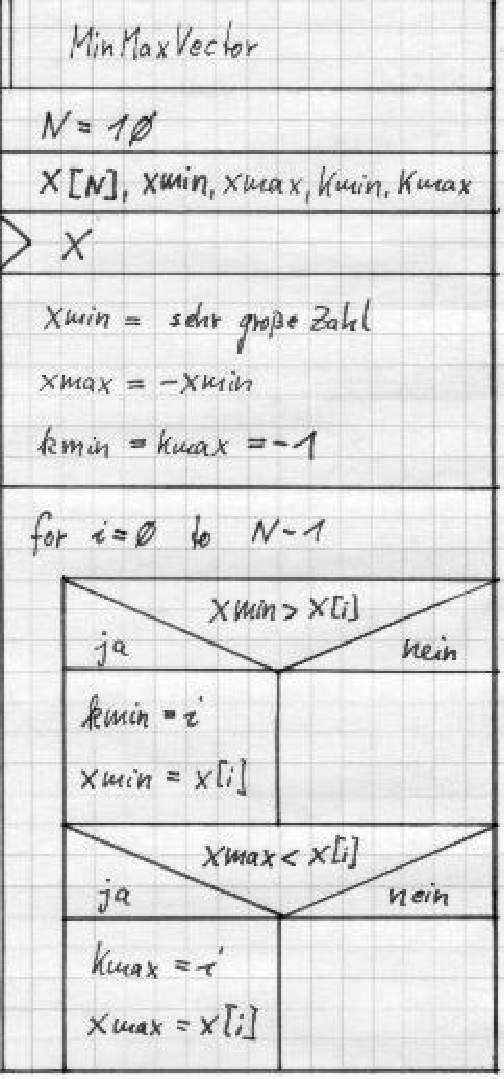
\includegraphics[scale=0.7]{GIF/p49a}
% 
% %
%  \item Vertausche Min/Max-Eintr"age. Bei Vektorl"ange~$0$ oder
%  	bei identischen Vektorelementen ist kein Vertauschen notwendig.
% \\
% %
% \underline{Struktogramm}: \\
% %begin{latexonly}
% %\begin{minipage}{0.4\textwidth}
% %\special{psfile=GIF/p49b.eps.gz
% %	 hscale=65 vscale=65
% %	 voffset=-130
% %	}
% %\mbox{}\\[4cm]
% %%\vspace{5.5cm}
% %\end{minipage}
% %\end{latexonly}
% %\htmladdimg{p49b_4.jpg}
% 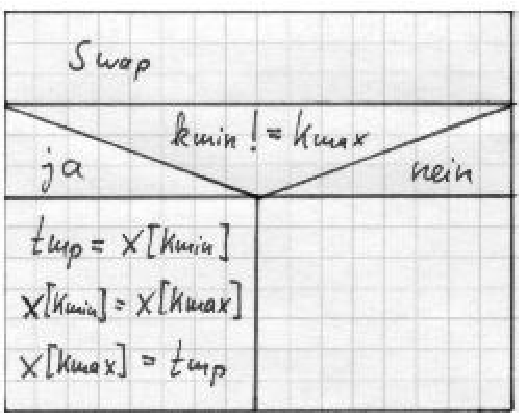
\includegraphics[scale=0.7]{GIF/p49b}
% %
% \hfill
% \begin{minipage}[b]{0.35\textwidth}
% Beim Vertauschen f"uhrt \\
% die naheliegende, erste Idee
% \verb| x[kmin] = x[kmax]| \\
% \verb| x[kmax] = x[kmin]| \\
% nicht zum Erfolg. Warum?
% \end{minipage}
% %
% \end{enumerate}
%%%%%%%%%%%%%%%%%%%%%%%%%%%%%%%%%%%%%%
\begin{minipage}[t]{0.45\textwidth}
  a) Bestimme Minimum und Maximum \\(und markiere die Positionen). \\[1ex]
%
 \underline{Struktogramm}: \\
 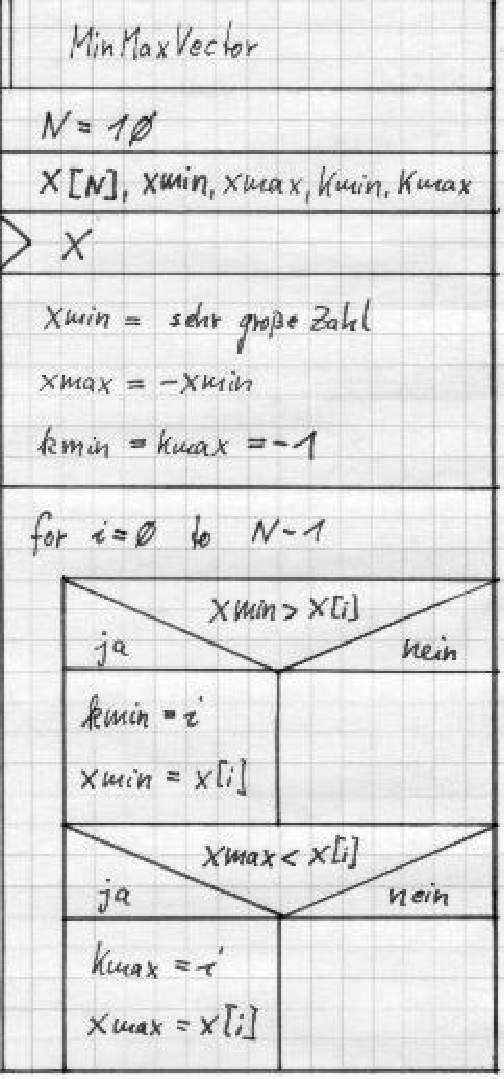
\includegraphics[scale=0.58]{GIF/p49a}
\end{minipage}
\hfill
\begin{minipage}[t]{0.45\textwidth}
 b) Vertausche Min/Max-Eintr"age. \\ Bei Vektorl"ange~$0$ oder
 	bei identischen Vektorelementen ist kein Vertauschen notwendig.
 	\\[1ex]
 %
\underline{Struktogramm}: \\
 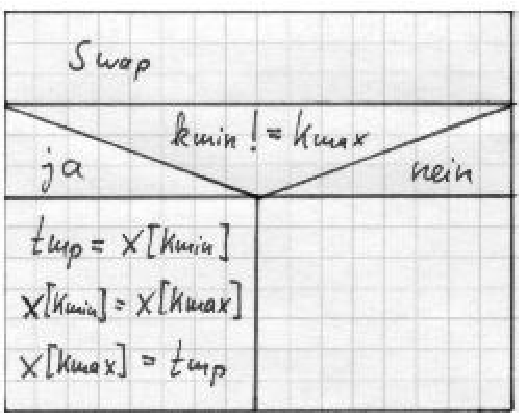
\includegraphics[scale=0.7]{GIF/p49b}
 \\[1ex]
 Beim Vertauschen f"uhrt \\
 die naheliegende, erste Idee
 \verb| x[kmin] = x[kmax]| \\
 \verb| x[kmax] = x[kmin]| \\
 nicht zum Erfolg. Warum?
\end{minipage}
%%%%%%%%%%%%%%%%%%%%%%%%%%%%%%%%%%%%%%
%
%
\includecode[linerange={7-16,27-49,60-61}]{bsp513.cpp}{Bestimme Min/Max eines Vektor und vertausche die Komponenten}
%
\index{numeric\_limits!max}\index{numeric\_limits}
In obigen beiden Listing wurden keine dynamischen Eigenschaften des Vektors benutzt,
daher hätten wir auch \verb|array<T,N>| verwenden können.
%
%
\subsection{Mehrdimensionale Felder in C++}
\label{p:5.1.4}
%
\subsubsection{Statische Matrizen}
\label{p:5.1.4.a}
%
%
Die Elemente der bisher betrachteten 1D-Felder sind im
Speicher hintereinander gespeichert (Modell des linearen Speichers), z.B,
wird der Zeilenvektor
\index{Feld!mehrdimensional}
\\[0.5ex]
\centerline{$\begin{pmatrix} x_0 & x_1 & x_2 & x_3 & x_4 \end{pmatrix}$}
\\
als
\\
%
\mbox{} \hfill\verb|double x[5];| \hfill\mbox{}
%
\\
vereinbart und gespeichert als
\\
%\centerline{\input{kap512a.pstex_t}}
\centerline{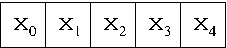
\includegraphics[scale=0.9]{kap512a.pdf}}
\\
wobei jede Zelle 8~Byte lang ist.

Ein zweidimensionales (statisches) Feld, z.B., eine Matrix~$A$ mit $N=4$~Zeilen
und $M=3$~Spalten
\index{Matrix}
\\[0.5ex]
\centerline{
$
A_{N \times M} :=
\begin{pmatrix}
 A_{00} & A_{01} & A_{02} \\
 A_{10} & A_{11} & A_{12} \\
 A_{20} & A_{21} & A_{22} \\
 A_{30} & A_{31} & A_{32}
\end{pmatrix}
$
}
\\[0.5ex]
kann im Speicher ebenfalls nur linear gespeichert werden, d.h.,
\\
% \centerline{\input{kap512b.pstex_t}}
\centerline{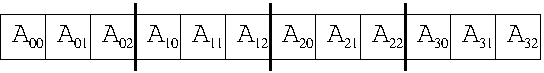
\includegraphics[scale=0.9]{kap512b.pdf}}
\\[0.5ex]
Daraus ergeben sich zwei M"oglichkeiten der 2D-Feldvereinbarung:
\begin{itemize}
 \item \underline{Variante 1 :} Als 2D-Feld.
%
\\[0.5ex]
\begin{minipage} {0.8\textwidth}
\begin{verbatim}
double A[N][M];               // Declaration in C
array<array<double,M>,N> A;   // Declaration in C++ (statisch)
A[3][1] = 5.0;                // Initialize A(3,1)
\end{verbatim}
\end{minipage}
%
 \item \underline{Variante 2 :} Als 1D-Feld.
 \label{page:2DarrayVariant2}
%
\\[0.5ex]
\begin{minipage} {0.8\textwidth}
\begin{verbatim}
double A[N*M];                // Declaration in C
array<double,M*N> A;          // Declaration in C++ (statisch)
A[3*M+1] = 5.0;               // Initialize A(3,1)
\end{verbatim}
\end{minipage}
%
\end{itemize}
%
\textbf{Beispiel}:  Als Beispiel betrachten wir die Multiplikation
der Matrix $A_{N \times M}$
bestehend aus $N=4$~Zeilen und $M=3$~Spalten
mit einem Zeilenvektor~$\underline{u}_M$
der L"ange~$M$.
Das Ergebnis ist ein Zeilenvektor~$\underline{f}_N$ der L"ange~$N$,
d.h., $\underline{f}_N : = A_{N \times M} \cdot \underline{u}_M$\enspace.
%
Die Komponenten von $\underline{f} = [f_0,f_1,\ldots,f_{N-1}]^T$
berechnen sich zu
%\bspfile{bsp514.cpp}
\begin{displaymath}
 f_i := \sum_{j=0}^{M-1} A_{i,j} \cdot u_j
 \qquad \forall i=0,\ldots,N-1 \enspace.
\end{displaymath}
In \emph{bsp514.cpp}\bspfile{bsp514.cpp} ist die Matrix in beiden Varianten
jeweils über ein C++-\texttt{array} implementiert.
\\
Deklariert man das 2D-Feld via \verb|array<array<T,MCOL>,NROW>| dann besteht
die Chance, daß die Matrixelemente linear im Speicher abgelegt werden.%
\index{Feld!statisch|)}
\index{Matrix}
%
\subsubsection{Dynamische Matrizen}
\label{p:5.1.4.b}
\index{Feld!dynamisch}
%
Die entsprechenden Realisierungen mit dem C++-\texttt{vector} sind
in \emph{bsp514\_b.cpp} verfügbar, wobei diese Implementierung
bei dynamischer Matrixgröße ihre Stärken ausspielt. 
%
Bei der Realisierung der Matrix als 2D-Feld via \verb|vector<vector<T>>| werden die
Matrixelemente nicht mehr linear im Speicher abgelegt und der Zugriff erfolgt wie in Variante~1.
%
\includecode[linerange={59-66}]{bsp514_b.cpp}{Dynamisches Allokieren einer Matrix}
%
\subsubsection{Dynamische Tensoren}
\label{p:5.1.4.c}
\index{Tensor}
H"oherdimensionale Felder k"onnen in Variante~1 analog zu Listing~\ref{lst:bsp514_b.cpp} 
deklariert und benutzt werden. 
In Variante~2 mu"s auf ein Element $B_{i,j,k}$ eines dreidimensionalen
Tensors  \verb| vector<double> B(L*N*M); | mittels \verb| B[i*M*N+j*M+k] | zugegriffen
werden.
%
%-----------------------------  if ----------------------------------------------------
\ifcteil                        %
\subsection{\mbox{}$^{*}$Statisches C-Array}
\label{sec:5.1.3}
%
In einem Feld werden Daten (Elemente) gleichen Typs zusammengefa"st.
Die allgemeine Vereinbarung eines statischen Feldes ist
\index{Feld!eindimensional}\index{Feld!statisch|(}
\\
\centerline{\texttt{ <typ> <bezeichner>[dimension];}}
%
wobei die eckigen Klammern ``['' und ``]''
unabdingbarer Bestandteil der Vereinbarung  sind.
Ein eindimensionales Feld entspricht mathematisch einem Vektor.
\index{Vektor}
%
\includecode[linerange={9-17,25-25,37-37}]{Ex510.cpp}{Statisches C-Array}

Die eckigen Klammern dienen im Vereinbarungsteil der Dimensionsvereinbarung
\verb|x[N]| und  im Anweisungsteil dem Zugriff auf einzelne
Feldelemente \verb|x[3]|\enspace.
Das Feld kann schon bei Deklaration initialisiert werden:
\index{Feld!Dimension}\index{Feld!Deklaration}\index{Feld!Initialisierung}
\\
\verb|double x[N] = {9,7,6,5,7}|

\underline{Achtung :} Die Numerierung der Feldelemente
beginnt mit 0. Daher darf nur auf Feldelemente
$x_i$, $i=0,\ldots,N-1$ zugegriffen werden.\index{Feld!Numerierung}\index{Feld!Feldelemente}
Andernfalls sind mysteri"oses Programmverhalten,
unerkl"arliche Fehlberechnungen und pl"otzliche Programmabst"urze
zu erwarten, deren Ursache nicht offensichtlich ist da
sie eventuell erst in weit entfernten Programmteilen auftreten k"onnen.
Diese Fehler müssen dann mit \emph{Memory-Checkern} mühsam gesucht werden, ein
gutes und freies Programm hierfür ist \texttt|valgrind| bzw.\
der \emph{inspector} in der Intel Toolbox.

Typischer Fehler

\begin{minipage} {0.95\textwidth}
\begin{verbatim}
//        Typical error
{
 const int N = 123;
       int ij[N] , i;
 ...
 for (i = 1; i <= N; ++i)    // !! WRONG !!
   {
     cout << ij[i] << endl;
   }
}
\end{verbatim}
\end{minipage}

\noindent
Es werden die Feldelemente $ij_1$, $ij_2$, $ij_3$, $ij_4$ und
der unsinnige Wert von $ij_5$ ausgegeben, jedoch  nicht das
allererste Feldelement $ij_0$\enspace.

Die Dimension eines statischen Feldes mu"s zum Zeitpunkt der
Compilierung bekannt sein, daher d"urfen nur Konstanten oder
aus Konstanten bestehende Ausdr"ucke als Dimension auftreten.
\index{Feld!statisch!Dimension}

\begin{minipage} {0.95\textwidth}
\begin{verbatim}
{
 const int N = 5, M = 1;
       int size;
 float x[5];            //  Correct
 short i[N];            //  Correct
 char  c[N-M+1];        //  Correct
 int   ij[size];        //  !! WRONG !!
}
\end{verbatim}
\end{minipage}

\textbf{Beispiel}:
Ein interessanter Spezialfall des Feldes ist die
Zeichenkette (String). Wir initialisieren den String mit
dem Wort ''Mathematik'' und  geben ihn in Normalschrift und
zeichenweise aus.\index{Feld!String}
%
\includecode[linerange={6-7,10-20,41-41}]{Ex511.cpp}{C-String als Spezialfall eines C-Arrays}
%

Die Zeichenkette h"atte auch mit
\\
\verb|char word[L] = "Mathematik";|
\\
oder
\\
\verb|char word[] = "Mathematik";|
\\
initialisiert werden k"onnen, wobei in letzterem Fall
die L"ange des Feldes \verb|word| aus der L"ange der
Zeichenkettenkonstante bestimmt wird.

% \pagebreak[4]
\textbf{Beispiel}:
Berechnung der $L_2$-Norm eines Vektors, d.h.,
$\parallel \underline{x} \parallel_{L_2} :=
 \sqrt{\sum\limits_{i=0}^{N-1} x_i^2}
$
%
\includecode[linerange={7-8,11-23,30-30}]{Ex512.cpp}{Berechnung der $L_{2}$-Norm eines Vektors}
%
%\pagebreak[4]

Als kleines \textbf{Beispiel} diene uns die Fibonacci Zahlenfolge,
welche "uber die zweistufige Rekursion\index{Fibonacci}
$$
f(n) _:= f(n-1) + f(n-2) \qquad n=2,\ldots
$$
mit den Anfangsbedingungen $f(0) = 0$, $f(1) = 1$ definiert ist.
%\exfile{Fibo1.cpp}
Zur Kontrolle k"onnen wir die
\ghref{http://de.wikipedia.org/wiki/Fibonacci-Folge\#Formel_von_Moivre-Binet}{Formel von Binet bzw.\  de Moivre}
%\htmladdnormallinkfoot{Formel von Binet bzw.\  de Moivre}
%{http://www.ee.surrey.ac.uk/Personal/R.Knott/Fibonacci/fibFormula.hpptml}
verwenden.
$$
f(n) = \frac{1}{\sqrt{5}}
 \left( \left(\frac{1+\sqrt{5}}{2}\right)^n
      - \left(\frac{1-\sqrt{5}}{2}\right)^n
 \right)
$$
%
\includecode[linerange={4-6,9-17,27-29,35-35}]{Fibo1.cpp}{Fibonacci numbers}
%

%\pagebreak[4]
Als weiteres \textbf{Beispiel} sollen Minimum und Maximum eines
Vektors bestimmt und die entsprechenden Vektorelemente
miteinander vertauscht werden (analog zu Pivotisierung).
%\exfile{Ex513.cpp}
Dies beinhaltet die beiden Teilaufgaben:
%
%
\begin{enumerate}
\renewcommand {\labelenumi}{\alph{enumi})}
 \item Bestimme Minimum und Maximum (und markiere die Positionen).
\\
%
\underline{Struktogramm}: \\
%\begin{latexonly}
%  \special{psfile=GIF/p49a.eps.gz
%	   hscale=65 vscale=65
%	   voffset=-340
%	}
%  \vspace{11.9cm}
%\end{latexonly}
%\htmladdimg{p49a_4.jpg}{}
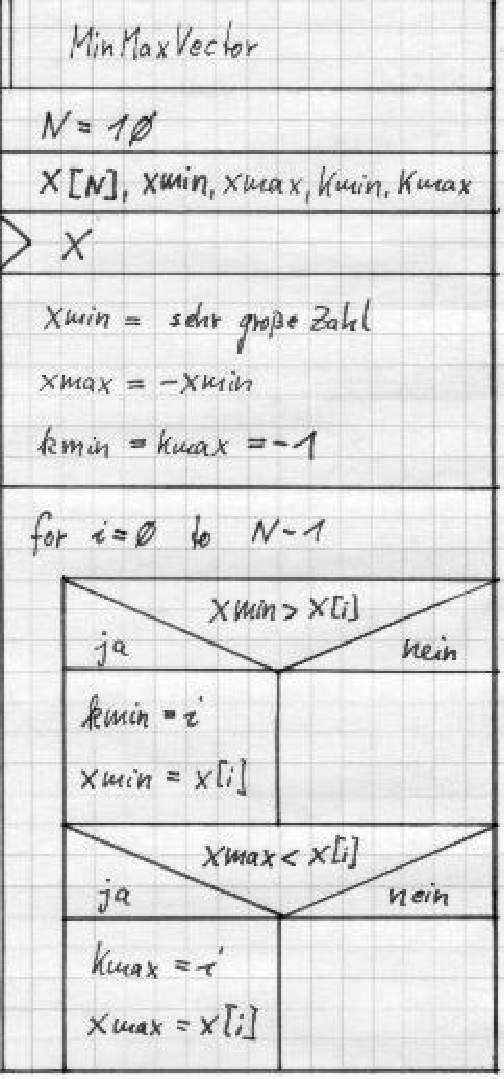
\includegraphics[scale=0.7]{GIF/p49a}

%
 \item Vertausche Min/Max-Eintr"age. Bei Vektorl"ange~$0$ oder
 	bei identischen Vektorelementen ist kein Vertauschen notwendig.
\\
%
\underline{Struktogramm}: \\
%begin{latexonly}
%\begin{minipage}{0.4\textwidth}
%\special{psfile=GIF/p49b.eps.gz
%	 hscale=65 vscale=65
%	 voffset=-130
%	}
%\mbox{}\\[4cm]
%%\vspace{5.5cm}
%\end{minipage}
%\end{latexonly}
%\htmladdimg{p49b_4.jpg}
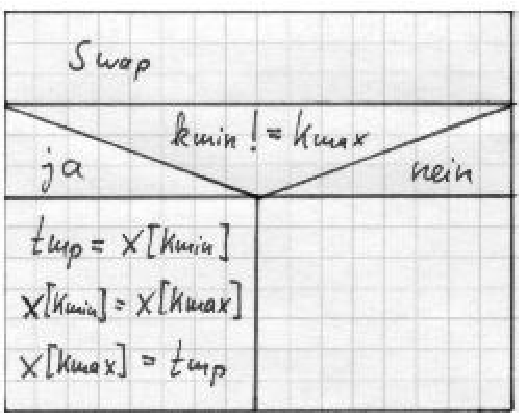
\includegraphics[scale=0.7]{GIF/p49b}
%
\hfill
\begin{minipage}[b]{0.35\textwidth}
Beim Vertauschen f"uhrt \\
die naheliegende, erste Idee
\verb| x[kmin] = x[kmax]| \\
\verb| x[kmax] = x[kmin]| \\
nicht zum Erfolg. Warum?
\end{minipage}
%
\end{enumerate}
%
\includecode[linerange={7-16,27-49,60-61}]{Ex513.cpp}{Bestimme Min/Max eines Vektor und vertausche die Komponenten}
%
\index{numeric\_limits!max}\index{numeric\_limits}
%
%
%
\subsection{\mbox{}$^{*}$Dynamisches C-Array}
\label{sec:5.1.4}
%
%
%
\subsection{\mbox{}$^{*}$Mehrdimensionale Felder}
\label{sec:5.1.5}
%
Die Eintr"age der bisher betrachteten 1D-Felder sind im
Speicher hintereinander gespeichert (Modell des linearen Speichers), z.B,
wird der Zeilenvektor
\index{Feld!mehrdimensional}
\\[0.5ex]
\centerline{$\begin{pmatrix} x_0 & x_1 & x_2 & x_3 & x_4 \end{pmatrix}$}
\\
als
\\
%
\mbox{} \hfill\verb|double x[5];| \hfill\mbox{}
%
\\
vereinbart und gespeichert als
\\
%\centerline{\input{kap512a.pstex_t}}
\centerline{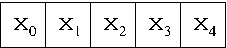
\includegraphics[scale=0.9]{kap512a.pdf}}
\\
wobei jede Zelle 8~Byte lang ist.

Ein zweidimensionales (statisches) Feld, z.B., eine Matrix~$A$ mit $N=4$~Zeilen
und $M=3$~Spalten
\index{Matrix}
\\[0.5ex]
\centerline{
$
A_{N \times M} :=
\begin{pmatrix}
 A_{00} & A_{01} & A_{02} \\
 A_{10} & A_{11} & A_{12} \\
 A_{20} & A_{21} & A_{22} \\
 A_{30} & A_{31} & A_{32}
\end{pmatrix}
$
}
\\[0.5ex]
kann im Speicher ebenfalls nur linear gespeichert werden, d.h.,
\\
% \centerline{\input{kap512b.pstex_t}}
\centerline{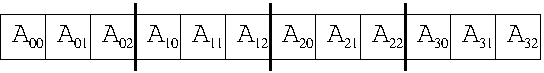
\includegraphics[scale=0.9]{kap512b.pdf}}
\\[0.5ex]
Daraus ergeben sich zwei M"oglichkeiten der 2D-Feldvereinbarung:
\begin{itemize}
 \item \underline{Variante 1 :} Als 2D-Array.
%
\\[0.5ex]
\begin{minipage} {0.8\textwidth}
\begin{verbatim}
double A[N][M];        // Declaration
A[3][1] = 5.0;         // Initialize A(3,1)
\end{verbatim}
\end{minipage}
%
 \item \underline{Variante 2 :} Als 1D-Array.
 \label{page:2DarrayVariant2}
%
\\[0.5ex]
\begin{minipage} {0.8\textwidth}
\begin{verbatim}
double A[N*M];         // Declaration
A[3*M+1] = 5.0;        // Initialize A(3,1)
\end{verbatim}
\end{minipage}
%
\end{itemize}
%
\textbf{Beispiel}:  Als Beispiel betrachten wir die Multiplikation
der Matrix $A_{N \times M}$
bestehend aus $N=4$~Zeilen und $M=3$~Spalten
mit einem Zeilenvektor~$\underline{u}_M$
der L"ange~$M$.
Das Ergebnis ist ein Zeilenvektor~$\underline{f}_N$ der L"ange~$N$,
d.h., $\underline{f}_N : = A_{N \times M} \cdot \underline{u}_M$\enspace.
%
Die Komponenten von $\underline{f} = [f_0,f_1,\ldots,f_{N-1}]^T$
berechnen sich zu
\bspfile{Ex514.cpp}
\begin{displaymath}
 f_i := \sum_{j=0}^{M-1} A_{i,j} \cdot u_j
 \qquad \forall i=0,\ldots,N-1 \enspace.
\end{displaymath}

H"oherdimensionale Felder k"onnen analog zu Version~1 deklariert und benutzt
werden. In Variante~2 mu"s auf ein Element $B(i,j,k)$ eines dreidimensionalen
Feldes  \verb| double B[L,N,M]; | mittels \verb| B[i*M*N+j*M+k] | zugegriffen
werden.
\index{Feld!statisch|)}
%----------------------------- fi ----------------------------------------------------
\fi                             %
%
%
%
%
%
\section{Liste}
\label{p:5.2}
%
Neben dem Vektor ist die Liste ein häufig benutztes Konstrukt zum
Speichern gleichartiger Argumente.
Auf Listen kann nicht, wie bei Vektoren, wahlfrei über einen Index zugegriffen werden
(also \verb|x[k]| geht nicht), sondern es muß auf die Listenelemente stets in
eine Richtung nacheinander zugegriffen werden.

Theoretisch sind Listen bei Sortieroperationen effizienter als Vektoren. 
Konkret hängt diese Aussage sehr stark vom Speicherbedarf der Elemente ab
da jedes Element einer Liste intern zusätzlich 2~Pointer benötigt 
und somit das Sortieren von Vektoren durch den geringeren Speicherdurchsatz schneller sein kann.
%%
%
\includecode[firstline=5]{bsp511b-list.cpp}{Berechnung mit einer Liste}
%
\begin{itemize}
    \item Zeile 7: Die Liste hat die Länge 0.
	\item Zeilen 8-13: Es werden solange Daten eingegeben, bis die Eingabegröße $<0$ ist. Dabei wächst die Liste
	in jedem Durchlauf um ein Element.
	\begin{itemize}
	  \item Zeile 11: Die Methode \ghref{http://www.cplusplus.com/reference/list/list/push_back/}{\texttt{push\_back}}
	  fügt den übergebenen Wert \texttt{tmp} als neues letztes Element an die Liste an.
	  \item Zeile 12: Die Methode \texttt{back} greift auf das aktuelle, letzte Element der Liste zu (und testet, ob
	  dieses nichtnegativ ist).
	  \item Zeile 13:  Die Methode \texttt{pop\_back} entfernt das negative letzte Element und verkürzt die Liste
	  entsprechend.
	\end{itemize}
	\item Zeile 15-17: For-Loop mit einem Iterator (\S\ref{p:6.3}) um auf die Listenelemente zuzugreifen:
    \begin{itemize}
        \item Zeile 15: Die Zuweisung \verb|auto pi=x.begin()| initialisiert die Laufvariable \verb|pi|
        mit dem Iterator auf das erste Listenelement.
        Der Typ von \verb|pi| wäre korrekterweise \verb|liste<double>::iterator|, das Schlüsselwort
        \verb|auto| erspart uns diesen Bandwurm und setzt den Typ automatisch korrekt.
        \item Zeile 16: \verb|*pi| stellt das aktuelle Listenelement dar
          (der Iterator muß dereferenziert werden).
    \end{itemize}
\end{itemize}

%
%
\section{Strukturen als einfache Klassen}
\label{p:5.3}
%
%
Die Struktur definiert einen neuen Datentyp welcher Komponenten
unterschiedlichen Typs vereint. Die Typdeklaration
\index{Struktur|(}

\mbox{}\hfill
\begin{minipage} {0.9\textwidth}
\begin{verbatim}
struct <struct_bezeichner>
 {
   <Datendeklaration>
 };
\end{verbatim}
\end{minipage}
\hfill\mbox{}

erlaubt die Deklaration von Variablen diesen Typs

\mbox{}\hfill
\begin{minipage} {0.9\textwidth}
\begin{verbatim}
<struct_bezeichner> <var_bezeichner>;
\end{verbatim}
\end{minipage}
\hfill\mbox{}

\textbf{Beispiel}: Wir deklarieren einen Datentyp zur Speicherung der
pers"onlichen Daten eines Studenten.
%
\includecode[linerange={4-21,27-29,33-36}]{bsp520.cpp}{Deklaration und Nutzung einer Struktur}
%
Die Zuweisung \verb| robbi = arni; | kopiert den kompletten Datensatz
von einer Variablen zur anderen. 
Dies funktioniert in Listing~\ref{lst:bsp520.cpp} automatisch, da z.B.\  
\verb| robbi.name = arni.name; | den erforderlichen Speicherplatz allokiert und den gesamten Inhalt des Strings kopiert.
Diese \emph{deep copy} funktioniert bei allen Standardatentypen und allen Containern der STL. 
%
\textbf{Achtung} bei Zeigern in der Struktur/Klasse. 
Hier muß die \emph{deep copy} selbst implementiert werden, da für die Zeiger nur eine \emph{shallow copy} sttattfindet, 
siehe dazu~\cite[p.~238f]{Breymann:2017:DCP}.
% siehe~\S~\textbf{XXXX}\ref{p:9_x} (\emph{deep} copy vs.\  \emph{shallow copy}).
%

\noindent
Der Zugriff auf die Komponente \verb|vorname| der Variablen \verb|arni|
(des Typs \verb|Student|) erfolgt "uber
%
% http://www.fredosaurus.com/notes-cpp/oop-condestructors/shallowdeepcopy.html
\\
\verb|arni.vorname|
\\[0.5ex]
%
Abgespeichert werden die Daten in der Form

% \input{kap520.pstex_t}
\centerline{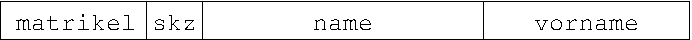
\includegraphics[scale=0.9]{kap520.pdf}}

Abh"angig von Compilereinstellungen bzw. -optionen k"onnen kleinere
ungenutzte Speicherl"ucken zwischen den Komponenten im Speicher auftreten
(Data Alignment f"ur schnelleren Datenzugriff).

Die Struktur \verb|Student| kann leicht f"ur Studenten, welche
mehrere Studienrichtungen belegen, erweitert werden.
%
\includecode[linerange={4-17,24-30,39-43}]{bsp520b.cpp}{Struktur  mit dynamischem Vektor als Komponente}
%

Die Struktur \verb|Student| enth"alt
bereits Felder als Komponenten. Andererseits k"onnen
diese Datentypen wiederum zu Feldern arrangiert werden.
\includecode[linerange={7-20,23-37,45-46}]{bsp522.cpp}{Dynamischem Vektor mit Strukturelementen}
%
\label{ex:522}

Strukturen k"onnen wiederum andere strukturierte Datentypen als
Komponenten enthalten.\index{Struktur!in Strukturen}
%
\includecode[linerange={7-26,35-36}]{bsp523.cpp}{Struktur mit Strukturkomponenten}

%

In obigem Beispiel ist \verb| line.p2 | eine Variable
vom Typ~\verb| Point3D |, auf deren  Daten wiederum mittels des
\verb| .|~Operators zugegriffen werden kann.
\index{Struktur|)}
%
%
%

\section{\mbox{}$^{*}$Union}
\label{p:5.4}
%
%
Alle Komponenten der Union werden auf dem gleichen Speicherbereich
"uberlappend abgebildet. Die Typdeklaration
\index{union}

\mbox{}\hfill
\begin{minipage} {0.5\textwidth}
\begin{verbatim}
union <union_bezeichner>
 {
   <Datendeklaration>
 };
\end{verbatim}
\end{minipage}
\hfill\mbox{}

erlaubt die Deklaration von Variablen diesen Typs

\mbox{}\hfill
\begin{minipage} {0.8\textwidth}
\begin{verbatim}
[union] <union_bezeichner> <var_bezeichner>;
\end{verbatim}
\end{minipage}
\hfill\mbox{}

Der Zugriff auf Komponenten der Union erfolgt wie bei einer Struktur.
%
%\includecode[linerange={7-26,35-36}]{Ex530.cpp}{Union}
\includecode[firstline=6]{Ex530.cpp}{Union}
%

\begin{minipage}[b]{0.55\textwidth}
Der Speicherplatzbedarf einer Union richtet sich nach der gr"o"sten
Komponente (hier \verb|sizeof(double)| = 8).
Die Union wird benutzt, um Speicherplatz zu sparen
bzw. tempor"are Felder f"ur verschiedene Datentypen zu "uberlagern,
sollte jedoch wegen der Fehlerm"oglichkeiten
erfahrenen Programmierern vorbehalten bleiben
(d.h. keine Verwendung im Praktikum).
\end{minipage}
\hfill
% \input{kap530.pstex_t}
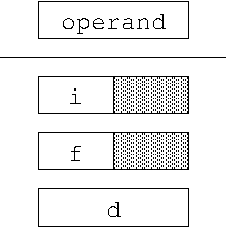
\includegraphics[scale=0.9]{kap530.pdf}
\hfill\mbox{}
%
%
%
%
\section{\mbox{}$^{*}$Aufzählungstyp}
\label{p:5.5}
%
%
Der Aufz"ahlungstyp ist ein Grundtyp mit frei w"ahlbarem Wertebereich,
dies sei an Hand der Wochentage veranschaulicht.
\index{Aufz\"ahlungstyp}
%
\includecode[linerange={6-27,40-41}]{Ex540.cpp}{Enumeration-Typ für Wochentage}
%
%
%
\section{\mbox{}$^{*}$Allgemeine Typvereinbarungen}
\label{p:5.6}
%
%
Die allgemeine Typdefinition

\mbox{}\hfill
\verb|typedef <type_definition> <type_bezeichner>|
\hfill\mbox{}

ist die konsequente
Weiterentwicklung zu frei definierbaren Typen.

Das nachfolgende Programmbeispiel illustriert die Definition
der drei neuen Typen \verb|Boolean|,  \verb|Text| und \verb|Point3D|.
%
\includecode[linerange={6-26,33-34}]{Ex550.cpp}{Typvereinbarungen}
%
%
Interessanterweise ist eine Variable vom Typ \verb|Text|
nunmehr stets eine Zeichenkettenvariable der (max.) L"ange~99.
Man beachte auch die Initialisierung der Variablen~\verb|p|.
Damit kann sogar eine Konstante vom Typ \verb|Point3d| deklariert
und initialisiert werden.

\underline{C++11}: Die neuere Möglichkeit der Definition eigener Typen nutzt \texttt{using}, 
z.B., in
%
\includecode[linerange={8-13}]{Ex550_11.cpp}{C++-11 Aliases}
%
